\newpage
\section{Quantum Wells}

Traveling Waves vs Standing Waves

On a stretched string we can set up both traveling waves and standing waves. 
\begin{itemize}
    \item A traveling wave, on a long string, can have any frequency. 
    \item A standing wave, set up on a string with a finite length, can have only discrete frequencies. 
\end{itemize}
In other words, confining the wave to a finite region of space leads to \highlight{quantization of the motion} --- to the existence of discrete states for the wave, each state with a sharply defined frequency.  

This observation appllies to waves of all kinds, including matter waves. For matter waves, however, it is more convenient to deal with the energy $E$ of the associated particle than the frequency $f$ of the wave. 

Consider the matter wave associated with an electron moving in the positive $x$ direction and subject to no net force --- a so-called \highlight{free particle}. The energe of such an electron can have any reasonable value, just as a wave traveling along a stretched string of infinite length can have any reasonable frequency. 

Consider next the matter wave associated with an atomic electron, perhaps the valence (least tightly bound) electron. The electron --- held within the atom by the attractive Coulomb force bewteen it and the positively charger nucleus --- is a \highlight{bound particle}. It can exist only in a set of discrete states, each having a discrete energy $E$. This sounds much like the discrete states and quantized frequencies that apply to a stretched string of finite length. 

For matter waves, then, as for all other kinds of waves, wa may state a confinement principle: \highlight{Confinement of a wave leads to quantization} --- that is, to the existence of discrete states with discrete energies. 

\quad

\subsection{An Electron in an Infinite Potential Well}

\subsubsection{One-Dimensional Infinite Potential Well}
Consider a nonrelativistic electron confined to a one-dimensional electron trap (or a limited region of space). 

\begin{figure}[H]
    \centering
    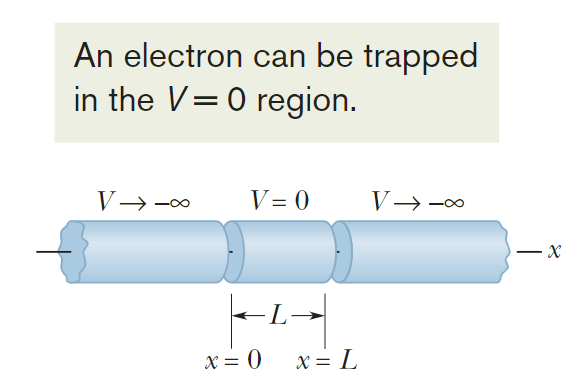
\includegraphics[width=0.309\textwidth]{Lec24/One-Dimensional Infinite Potential Well}
    \caption{One-Dimensional Infinite Potential Well}
\end{figure}

The trap consists of two semi-infinitely long cylinders, each of which has an electric potential approaching $-\infty$; bewteen them is a hollow cylinders of length $L$, which has an electric potential of zero. We put a single electron into this central cylinder to trap it. 

\begin{figure}[H]
    \centering
    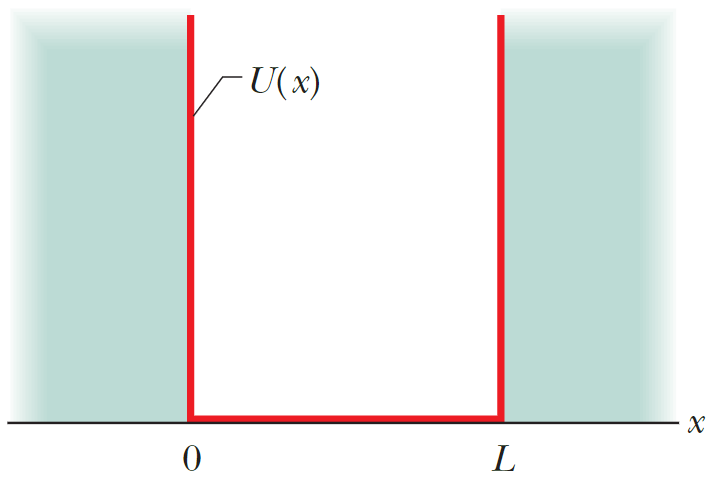
\includegraphics[width=0.309\textwidth]{Lec24/1D Trap}
    \caption{1D Trap}
\end{figure}

When the electron is in the central cylinder, its potential energy $U=-eV$ is zero. If the electron couldn't get out of this region, its potential energy would be positively infinite outside. It is a potential ``well'' because an electron placed in the central cylinder cann't escape from it. 

\subsubsection{Standing Waves in a 1D Trap}
We examine \highlight{by analogy with standing waves on a string} of finite length, stretched along an $x$ axis and confined bewteen rigid supports. Because the supports are rigid, the two ends of the string are nodes, or points at which the string is always at rest. The states, or discrete standing wave patterns in which the string can oscillate, are those for which the length $L$ of the string is equal to an integer number of half-wavelengths; that is, the string can occupy only states for which
\begin{align*}
    L=\frac{n\lambda}{2}\,\text{for}\,n=1,2,3,\dots
\end{align*}
Each value of the integer $n$ identifies a state of the oscillating string. 

For a given $n$, the transverse displacement of the string at any position $x$ along the string is given by 
\begin{align*}
    y_n(x)=A\sin\left( \frac{n\pi}{L} x\right)
\end{align*}
where A is the amplitude of the standing wave. For the electron in the trap, we promote the transverse displacement to wave function $\psi_n(x)$. 

\subsubsection{Probability of Detection}
Classically, we expect to detect the electron anywhere in the infinite well with a constant probability density. Quantum mechanically, we find the probability density 
\begin{align*}
    P_n(x)=|\psi_n(x)|^2=|A|^2\sin^2\left(\frac{n\pi}{L}x\right)
\end{align*}
for a given $n$. The constant $A$ (up to a phase) can be determined by the \highlight{normalization} condition
\begin{align*}
    \int_{-\infty}^{\infty}|\psi_n(x)|^2\,\mathrm{d}x=\int_0^L|\psi_n(x)|^2\,\mathrm{d}x=1
\end{align*}
so $A=\sqrt{\frac{2}{L}}$

\subsubsection{Energies of the Trapped Electron}
The de Broglie wavelength $\lambda$ of the electron is defined as 
\begin{align*}
    \lambda=\frac{h}{p}=\frac{h}{\sqrt{2mK}}=\frac{2L}{n}
\end{align*}
where $K=\frac{p^2}{2m}$ is the kinetic energy of the nonrelativistic electron. 

For an electron moving within the central cylinder, where $U=0$, the total (mechanical) energy $E$ is equal to the kinetic energy $K$. Thereforce, the tota energy for an electron moving in the central cylinder is 
\begin{align*}
    E_n=\frac{h^2}{8mL^2}n^2
\end{align*}
for $n=1,2,3,\dots$. 

The positive integer $n$ here is the \highlight{quantum number} of the electron quantum state in the trap. The quantum state with the lowest possible energy level $E_1$ with quantum number $n=1$ is called the \highlight{ground state} of the electron. 

\begin{figure}[H]
    \centering
    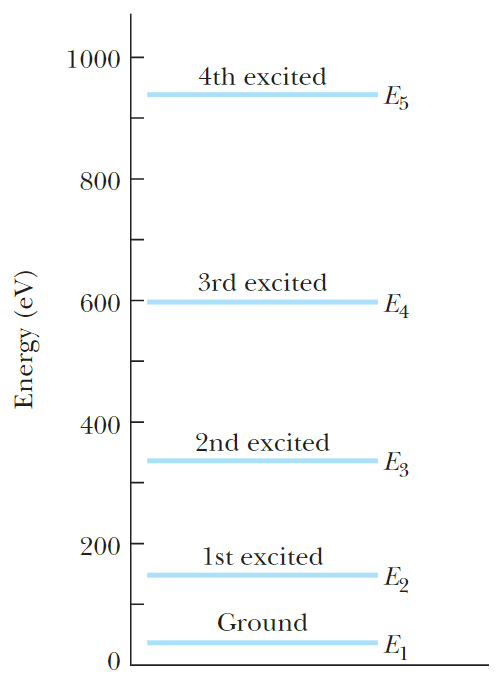
\includegraphics[width=0.22\textwidth]{Lec24/the total energy for an electron moving in the central cylinder}
    \caption{the total energy for an electron moving in the central cylinder}
\end{figure}

\highlight{Why is $n=0$ not allowed?} Choosing $n=0$ would indeed yield a lower energy of zero. However, as we will see below the corresponding probability density is $|\psi|=0$, which we can interpret only to mean that there is no electron in the well; so $n=0$ is not a possible quantum number. It is an important conclusion of quantum physics that \highlight{confined systems must always have a certain minimum energy} called the \highlight{zero-point energy}. 

Electrons can be excited or de-excited by the absorption or emission of a photon with energy
\begin{align*}
    \hbar\omega=\frac{hc}{\lambda}=\Delta E=E_{high}-E_{low}
\end{align*}

\begin{figure}[H]
    \centering
    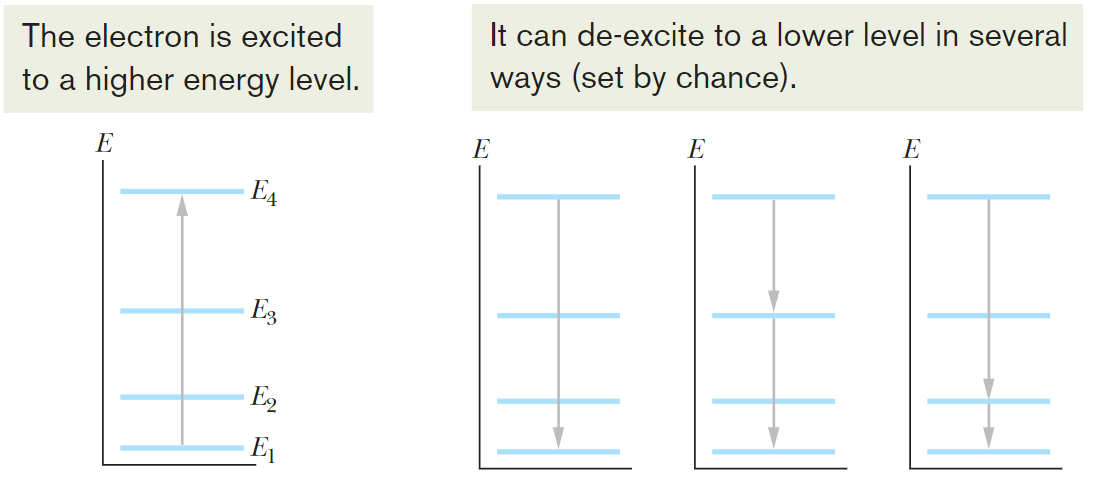
\includegraphics[width=0.309\textwidth]{Lec24/excited and de-excited}
    \caption{excited and de-excited}
\end{figure}

\subsubsection{Wave Function of the Trapped Electron}
If we solve Schroedinger's equation, for an electron trapped in the 1D infinite well of width $L$, we could write the solutions as 
\begin{align*}
    \psi_n(x)=&e^{ikx} \\
    \text{or}\,\psi_n(x)=&e^{-ikx}\\
    k=\frac{2\pi}{\lambda}=&\frac{n\pi}{L}
\end{align*}
However, the traveling waves don't satisfy the boundary conditions
\begin{align*}
    \psi_n(0)=\psi_n(L)=0
\end{align*}

The appropriated solutions can only be certain linear combinations of the traveling wave functions, given by 
\begin{align*}
    \psi_n(x)=A\sin(kx)
\end{align*}
for $0\le x\le L$. The constant $A$ is to be determined. Note that the wave functions $\psi_n(x)$ have the same form as the displacement functions $y_n(x)$ for a standing  wave on a string stretched bewteen rigid supports. 

\begin{figure}[H]
    \centering
    \begin{subfigure}{0.22\textwidth}
        \centering
        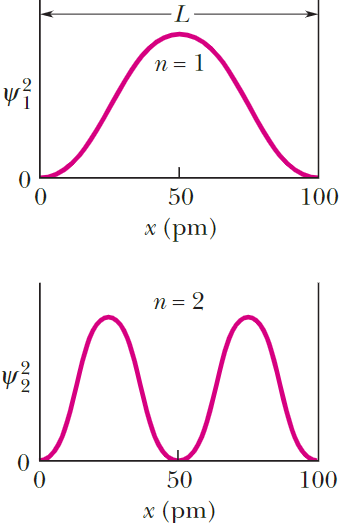
\includegraphics[width=\textwidth]{Lec24/The probability density for 1}
    \end{subfigure}
    \begin{subfigure}{0.22\textwidth}
        \centering
        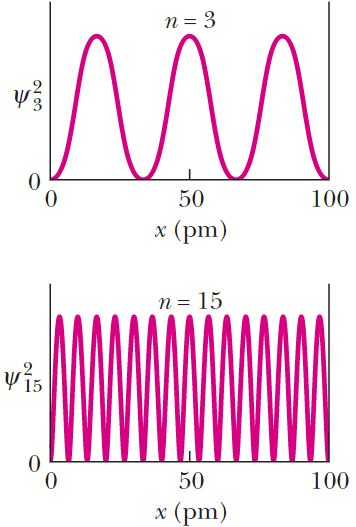
\includegraphics[width=\textwidth]{Lec24/The probability density for 2}
    \end{subfigure}
    \caption{The probability density for n=1,2,3,15}
\end{figure}

For sufficiently large $n$, the probability of detection becomes more and more uniform across the well. This result is an instance of a general principle called the \highlight{correspondence principle: At large enough quantum numbers, the predictions quantum physics merge smoothly with those of classical physics}. 

\subsection{An Electron in a Finite Potential Well}
We can picture an electron trapped in a one-\\dimensional well between infinite-potential walls as being a standing matter wave. The solutions must be zero at the infinite walls. For finite walls, however, the analogy bewteen waves on a stretched string and matter waves fails. Matter wave nodes no longer exist at $x=0$ and at $x=L$; wave function can penetrate the walls into \highlight{classically forbidden} regions. 

To find the wave function describing the quantum states of an electron in a finite well, we must resort to the time-independent Schroedinger's equation
\begin{align*}
    -\frac{\hbar^2}{2m}\frac{\partial^2\psi(x)}{\partial x^2}+U(x)\psi(x)=E\psi(x)
\end{align*}

Rather than solving this equation for the finite well, much alike what we did in the case of a potential barrier, we proceed with a qualitative discussions. 

\begin{figure}[H]
    \centering
    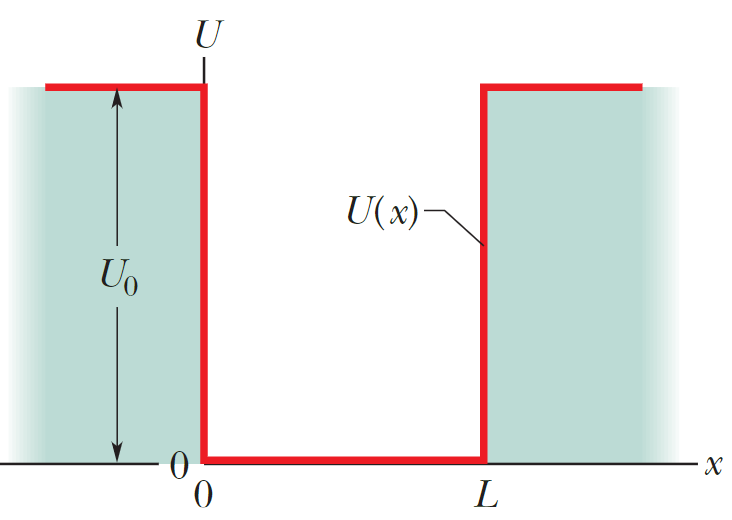
\includegraphics[width=0.309\textwidth]{Lec24/An Electron in a Finite Potential Well}
    \caption{An Electron in a Finite Potential Well}
\end{figure}

\subsubsection[Wave Functions of the Trapped Ele-ctron]{Wave Functions of the Trapped Electron}
As in the tunneling problem, the matter wave ``leaks'' into the walls of a finite potential energy well; the leakage is greater for greater value of quantum number $n$. As a result, the wavelength $\lambda$ for any given quantum state is greater when teh electron is trapped in a finite well than when it is trapped in an infinite well of the same length $L$. 

\subsubsection{Energies of the Trapped Electron}
Thus, the corresponding energy $E=\frac{\frac{h}{\lambda}^2}{2m}$ for an electron in any given state is less in the finite well than in the infinite well. An electrons with an energy greater than the well depth has too much energy to be trapped in the finite well. Thus, there is \highlight{a continuum of energies beyond the top of the well}; a high-energy electron is not confined, and its energy isn't quantized. 

\begin{figure}[H]
    \centering
    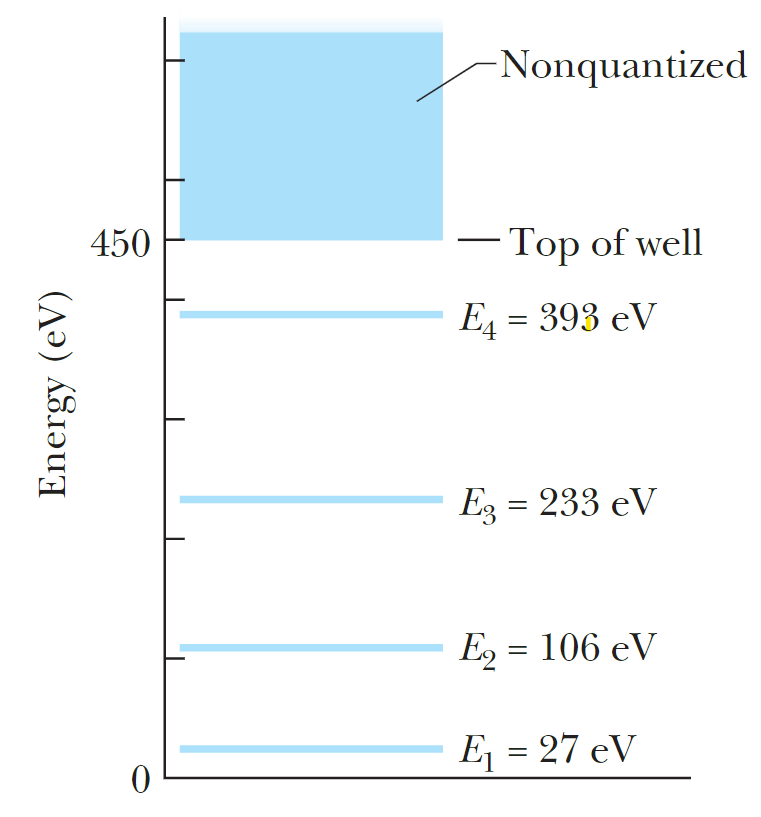
\includegraphics[width=0.129\textwidth]{Lec24/an electron in the finite well}
    \caption{an electron in the finite well}
\end{figure}

\subsection{High Dimensional Electron Traps}

\subsubsection{Schroedinger's Equation in High Dimensions}
Assuming $U=0$. We can generalize Schroedinger's equation to 2D (and similarly to 3D) as 
\begin{align*}
    E\Psi(x,y)=-\frac{\hbar^2}{2m}\left[ \frac{\partial^2}{\partial x^2}+\frac{\partial^2}{\partial y^2} \right]\Psi(x,y)
\end{align*}

We are interested in a family of wave functions $\Psi(x,y)=X(x)Y(y)$, whose Schroedinger's equation is equivalent to 
\begin{align*}
    E=-\frac{\hbar^2}{2m}\frac{1}{X(x)}\frac{\partial^2 X(x)}{\partial x^2}-\frac{\hbar^2}{2m}\frac{1}{Y(y)}\frac{\partial^2 Y(y)}{\partial y^2}
\end{align*}

This has the form $E=F(x)+G(y)$, which can only be satisfied when $F(x)=E_1$ and $G(y)=E-E_1$, i.e. each function must separately be a constant. As a consequence, separation of variables breaks the multivariate partial differential equation into a set of independent ordinary differential equations (ODEs). We can solve the ODEs for $X (x )$ and $Y (y )$. The wave function for the original equation is simply their product $X (x )Y (y )$. Success requires choice of an appropriate coordinate system and may not be attainable at all depending on the equation.

\subsubsection{2D \& 3D Infinite Potential Wells}

\begin{figure}[H]
    \centering
    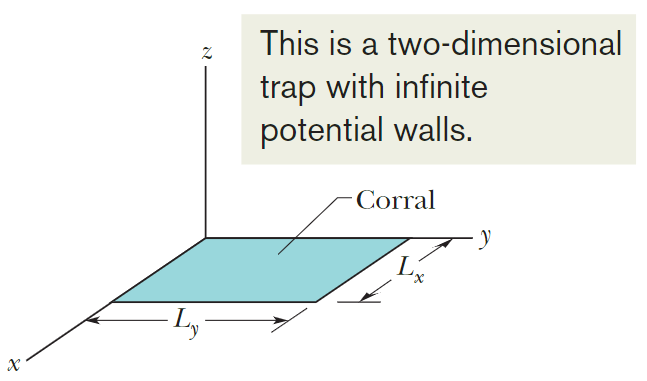
\includegraphics[width=0.309\textwidth]{Lec24/2D infinite potential}
    \caption{2D infinite potential well}
\end{figure}

Consider a 2D infinite potential well of widths $L_x$ and $L_y$ (e.g. for an electron on a surface). The normalized wave function are
\begin{align*}
    \psi_n(x,y)=&\frac{2}{\sqrt{L_x L_y}}\sin (k_x x)\sin(k_y y)\\
    k_x=&\frac{2\pi}{\lambda_x}=\frac{n_x \pi}{L_x}\\
    k_y=&\frac{2\pi}{\lambda_y}=\frac{n_y \pi}{L_y}
\end{align*}
with two quantum numbers $n_x$ and $n_y$, and the corresponding energies are
\begin{align*}
    E_{n_x,n_y}=\frac{h^2}{8m}\left(\frac{n_x^2}{L_x^2}+\frac{n_y^2}{L_y^2}\right)
\end{align*}

\begin{figure}[H]
    \centering
    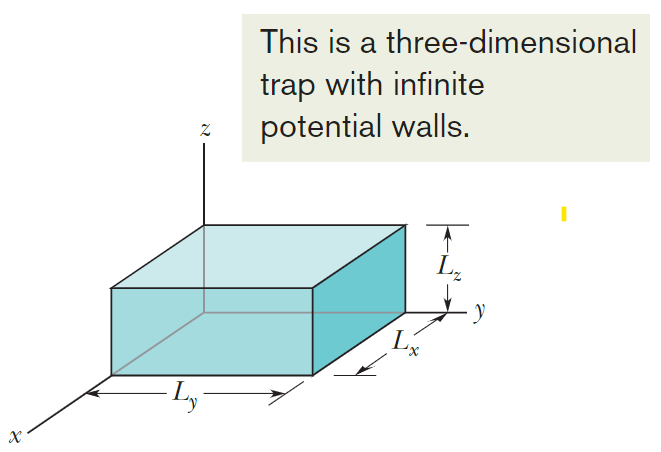
\includegraphics[width=0.309\textwidth]{Lec24/a 3D infinite potential well}
    \caption{a 3D infinite potential well}
\end{figure}

An electrons can also be trapped in a 3D infinite potential well with a volume $V=L_x L_y L_z$. Now a trapped electron has three quantum numbers $n_x$, $n_y$ abd $n_z$. The normalized wave function and their energies are
\begin{align*}
    \psi_n(x,y,z)=&\sqrt{\frac{8}{V}}\sin (k_x x) \sin (k_z z) \sin (k_z z)\\
    k_x=&\frac{n_x \pi}{L_x},\,k_y=\frac{n_y \pi}{L_y},\,k_z=\frac{n_z \pi}{L_z} \\
    E_{n_x,n_y,n_z}=&\frac{h^2}{8m}\left(\frac{n_x^2}{L_x^2}+\frac{n_y^2}{L_y^2}+\frac{n_z^2}{L_z^2}\right)
\end{align*}